% !TeX spellcheck = de_DE
\documentclass[portrait,final,a2paper,fontscale=0.79]{baposter}

%
% TODO: You may use fontscale to adjust the font size so that the poster fills the whole page.
%

%\usepackage[ngerman]{babel}
\usepackage[english]{babel}
%\usepackage{fixltx2e}
\usepackage{babelbib}
\usepackage[utf8]{inputenc}

\usepackage{calc}
\usepackage{graphicx}
\usepackage{amsmath}
\usepackage{amssymb}
\usepackage{relsize}
\usepackage{multirow}
\usepackage{rotating}
\usepackage{bm}
\usepackage{url}

\usepackage{graphicx}
\usepackage{multicol}

%\usepackage{times}
\usepackage{helvet}
%\usepackage{bookman}
\usepackage{palatino}

\usepackage{floatflt}

\usepackage{mwe} % for example images
\usepackage{blindtext}

\newcommand{\captionfont}{\footnotesize}

\graphicspath{{images/}{../images/}}
\usetikzlibrary{calc}

%%%%%%%%%%%%%%%%%%%%%%%%%%%%%%%%%%%%%%%%%%%%%%%%%%%%%%%%%%%%%%%%%%%%%%%%%%%%%%%%
% Multicol Settings
%%%%%%%%%%%%%%%%%%%%%%%%%%%%%%%%%%%%%%%%%%%%%%%%%%%%%%%%%%%%%%%%%%%%%%%%%%%%%%%%
\setlength{\columnsep}{1.5em}
\setlength{\columnseprule}{0mm}

%%%%%%%%%%%%%%%%%%%%%%%%%%%%%%%%%%%%%%%%%%%%%%%%%%%%%%%%%%%%%%%%%%%%%%%%%%%%%%%%
% Save space in lists. Use this after the opening of the list
%%%%%%%%%%%%%%%%%%%%%%%%%%%%%%%%%%%%%%%%%%%%%%%%%%%%%%%%%%%%%%%%%%%%%%%%%%%%%%%%
\newcommand{\compresslist}{%
\setlength{\itemsep}{1pt}%
\setlength{\parskip}{0pt}%
\setlength{\parsep}{0pt}%
}

%%%%%%%%%%%%%%%%%%%%%%%%%%%%%%%%%%%%%%%%%%%%%%%%%%%%%%%%%%%%%%%%%%%%%%%%%%%%%%
%%% Begin of Document
%%%%%%%%%%%%%%%%%%%%%%%%%%%%%%%%%%%%%%%%%%%%%%%%%%%%%%%%%%%%%%%%%%%%%%%%%%%%%%

\begin{document}

%%%%%%%%%%%%%%%%%%%%%%%%%%%%%%%%%%%%%%%%%%%%%%%%%%%%%%%%%%%%%%%%%%%%%%%%%%%%%%
%%% Here starts the poster
%%%---------------------------------------------------------------------------
%%% Format it to your taste with the options
%%%%%%%%%%%%%%%%%%%%%%%%%%%%%%%%%%%%%%%%%%%%%%%%%%%%%%%%%%%%%%%%%%%%%%%%%%%%%%
% Define some colors

%\definecolor{lightblue}{cmyk}{0.83,0.24,0,0.12}
%\definecolor{lightblue}{rgb}{0.145,0.6666,1}

% HSA-Farben
\definecolor{hsa_himbeerrot}{RGB}{205,0,69}
\definecolor{hsa_reinorange}{RGB}{255,101,0}
\definecolor{hsa_blau}{RGB}{29,96,210}
\definecolor{hsa_hellgrau}{RGB}{161,153,144}
\definecolor{hsa_dunkelgrau}{RGB}{98,98,103}

\begin{poster}%
  % Poster Options
  {
  % Show grid to help with alignment
  grid=false,
  columns=2,
  % Column spacing
  colspacing=1em,
  % Color style
  bgColorOne=white,
  bgColorTwo=hsa_hellgrau,
  borderColor=hsa_reinorange,
  headerColorOne=hsa_reinorange,
  headerColorTwo=hsa_himbeerrot,
  headerFontColor=white,
  boxColorOne=white,
  boxColorTwo=hsa_reinorange,
  % Format of textbox
  %textborder=roundedleft,
  textborder=bars,
  % Format of text header
  eyecatcher=true,
  headerborder=closed,
  headerheight=0.1\textheight,
%  textfont=\sc, An example of changing the text font
  headershape=rectangle,
  headershade=plain,
  headerfont=\Large\bf\sc, %Sans Serif
  textfont={\sf\setlength{\parindent}{1.5em}},
  boxshade=plain,
%  background=shade-tb,
  background=plain,
  linewidth=2pt
  }
  % Eye Catcher
  {
	
\includegraphics[height=7.5em]{images/talking_machines_logo.png}
  } 
  % Title
  {\bf\textsc{Talking Machines}\vspace{0.5em}}
  % Subtitle
  {\bf\textsc{Voice assistant for machine interaction in Industry 4.0}\vspace{0.5em}}
  % University logo
  {% The makebox allows the title to flow into the logo, this is a hack because of the L shaped logo.
    %\includegraphics[height=9.0em]{images/logo}
    
\includegraphics[height=7em]{images/hsa_logo_normal.jpg}
  }	
%%%%%%%%%%%%%%%%%%%%%%%%%%%%%%%%%%%%%%%%%%%%%%%%%%%%%%%%%%%%%%%%%%%%%%%%%%%%%%
%%% Now define the boxes that make up the poster
%%%---------------------------------------------------------------------------
%%% Each box has a name and can be placed absolutely or relatively.
%%% The only inconvenience is that you can only specify a relative position 
%%% towards an already declared box. So if you have a box attached to the 
%%% bottom, one to the top and a third one which should be in between, you 
%%% have to specify the top and bottom boxes before you specify the middle 
%%% box.
%%%%%%%%%%%%%%%%%%%%%%%%%%%%%%%%%%%%%%%%%%%%%%%%%%%%%%%%%%%%%%%%%%%%%%%%%%%%%%

%%%%%%%%%%%%%%%%%%%%%%%%%%%%%%%%%%%%%%%%%%%%%%%%%%%%%%%%%%%%%%%%%%%%%%%%%%%%%%
\headerbox{Motivation / State of the Art}{name=problem,column=0,row=0}{
%%%%%%%%%%%%%%%%%%%%%%%%%%%%%%%%%%%%%%%%%%%%%%%%%%%%%%%%%%%%%%%%%%%%%%%%%%%%%%
Today we are in the fourth industrial revolution or also known as Industry 4.0, where virtual 
and physical manufacturing systems cooperation intensifies on a global level 
(Pistorius, 2020, p.5). \\

Meanwhile the recent advancements in AI offer significant chances for the improvement and extended use 
of virtual assistants. As it is the basis for natural language processing (NLP), 
a key technology part of chatbots utilized to understand the human language (Market Research Future, 2021).\\

There are many virtual assistants on the market for home automation and personal tasks (Petrock, 2020). 
But the global voice assistant market is still expected to grow significantly in the next 5 years. 
One of the key drivers in Europe for this development is the adaptation of voice-based-solutions 
in the industrial sector (Market Research Future, 2021). 
}


%%%%%%%%%%%%%%%%%%%%%%%%%%%%%%%%%%%%%%%%%%%%%%%%%%%%%%%%%%%%%%%%%%%%%%%%%%%%%%
\headerbox{Goal}{name=goal,column=0,row=0, below=problem}{
%%%%%%%%%%%%%%%%%%%%%%%%%%%%%%%%%%%%%%%%%%%%%%%%%%%%%%%%%%%%%%%%%%%%%%%%%%%%%%
Our project aimed to explore the chances of voice assistants for Industry 4.0 in HEKUMA machines, 
as this project is an industry cooperation between the HEKUMA GmbH and the HSA. 
The HEKUMA GmbH is a leading special machine construction company from the Munich area. \\

The overall goal was archived by first researching the state of the art, 
evaluating different approaches, and then choosing a fitting framework for a future prototype. 
Next the architecture of that said prototype was designed and later implemented. 
During this process we oriented ourselves on, example conversations provided by the HEKUMA GmbH. 
Adapted versions of those can be seen in the “Results” section below.
}

%%%%%%%%%%%%%%%%%%%%%%%%%%%%%%%%%%%%%%%%%%%%%%%%%%%%%%%%%%%%%%%%%%%%%%%%%%%%%%
\headerbox{Architecture}{name=architecture,column=0,span=1,below=goal}{
%%%%%%%%%%%%%%%%%%%%%%%%%%%%%%%%%%%%%%%%%%%%%%%%%%%%%%%%%%%%%%%%%%%%%%%%%%%%%%
The design of our concept is based around the Rasa framework. 
Rasa was chosen amongst other reasons for the fact that it can run locally on the machine without needing to have an internet connection. 
With a very limited amount of training data in the form of classified example sentences, 
Rasa makes it very easy to analyze intents, extract entities and connect them to answers or possible actions. 
These actions are defined through Rasa Actions and make it possible for us to attach our chatbot to an industrial machine. \\

As we were only supposed to develop a prototype, the industrial machine in our case is only represented by an ativse server. 
It contains information about the state of an imaginary machine, with alarm values and other important operating information. 
Changing values on this atvise server does, at this stage, not lead to any changes on a real machine. But it was incredibly useful for prototyping. \\

The atvise server exchanges data with our Rasa actions server through OPC UA. OPC UA is a machine to machine communication protocol.
Therefore, our Rasa actions server needs to understand this form of communication. This was made possible by using the library opcua-asyncio.
opcua-asyncio is a Python 3 library and worked perfectly well with our actions Rasa actions server, which also needs to be written in Python. 
\begin{center}
	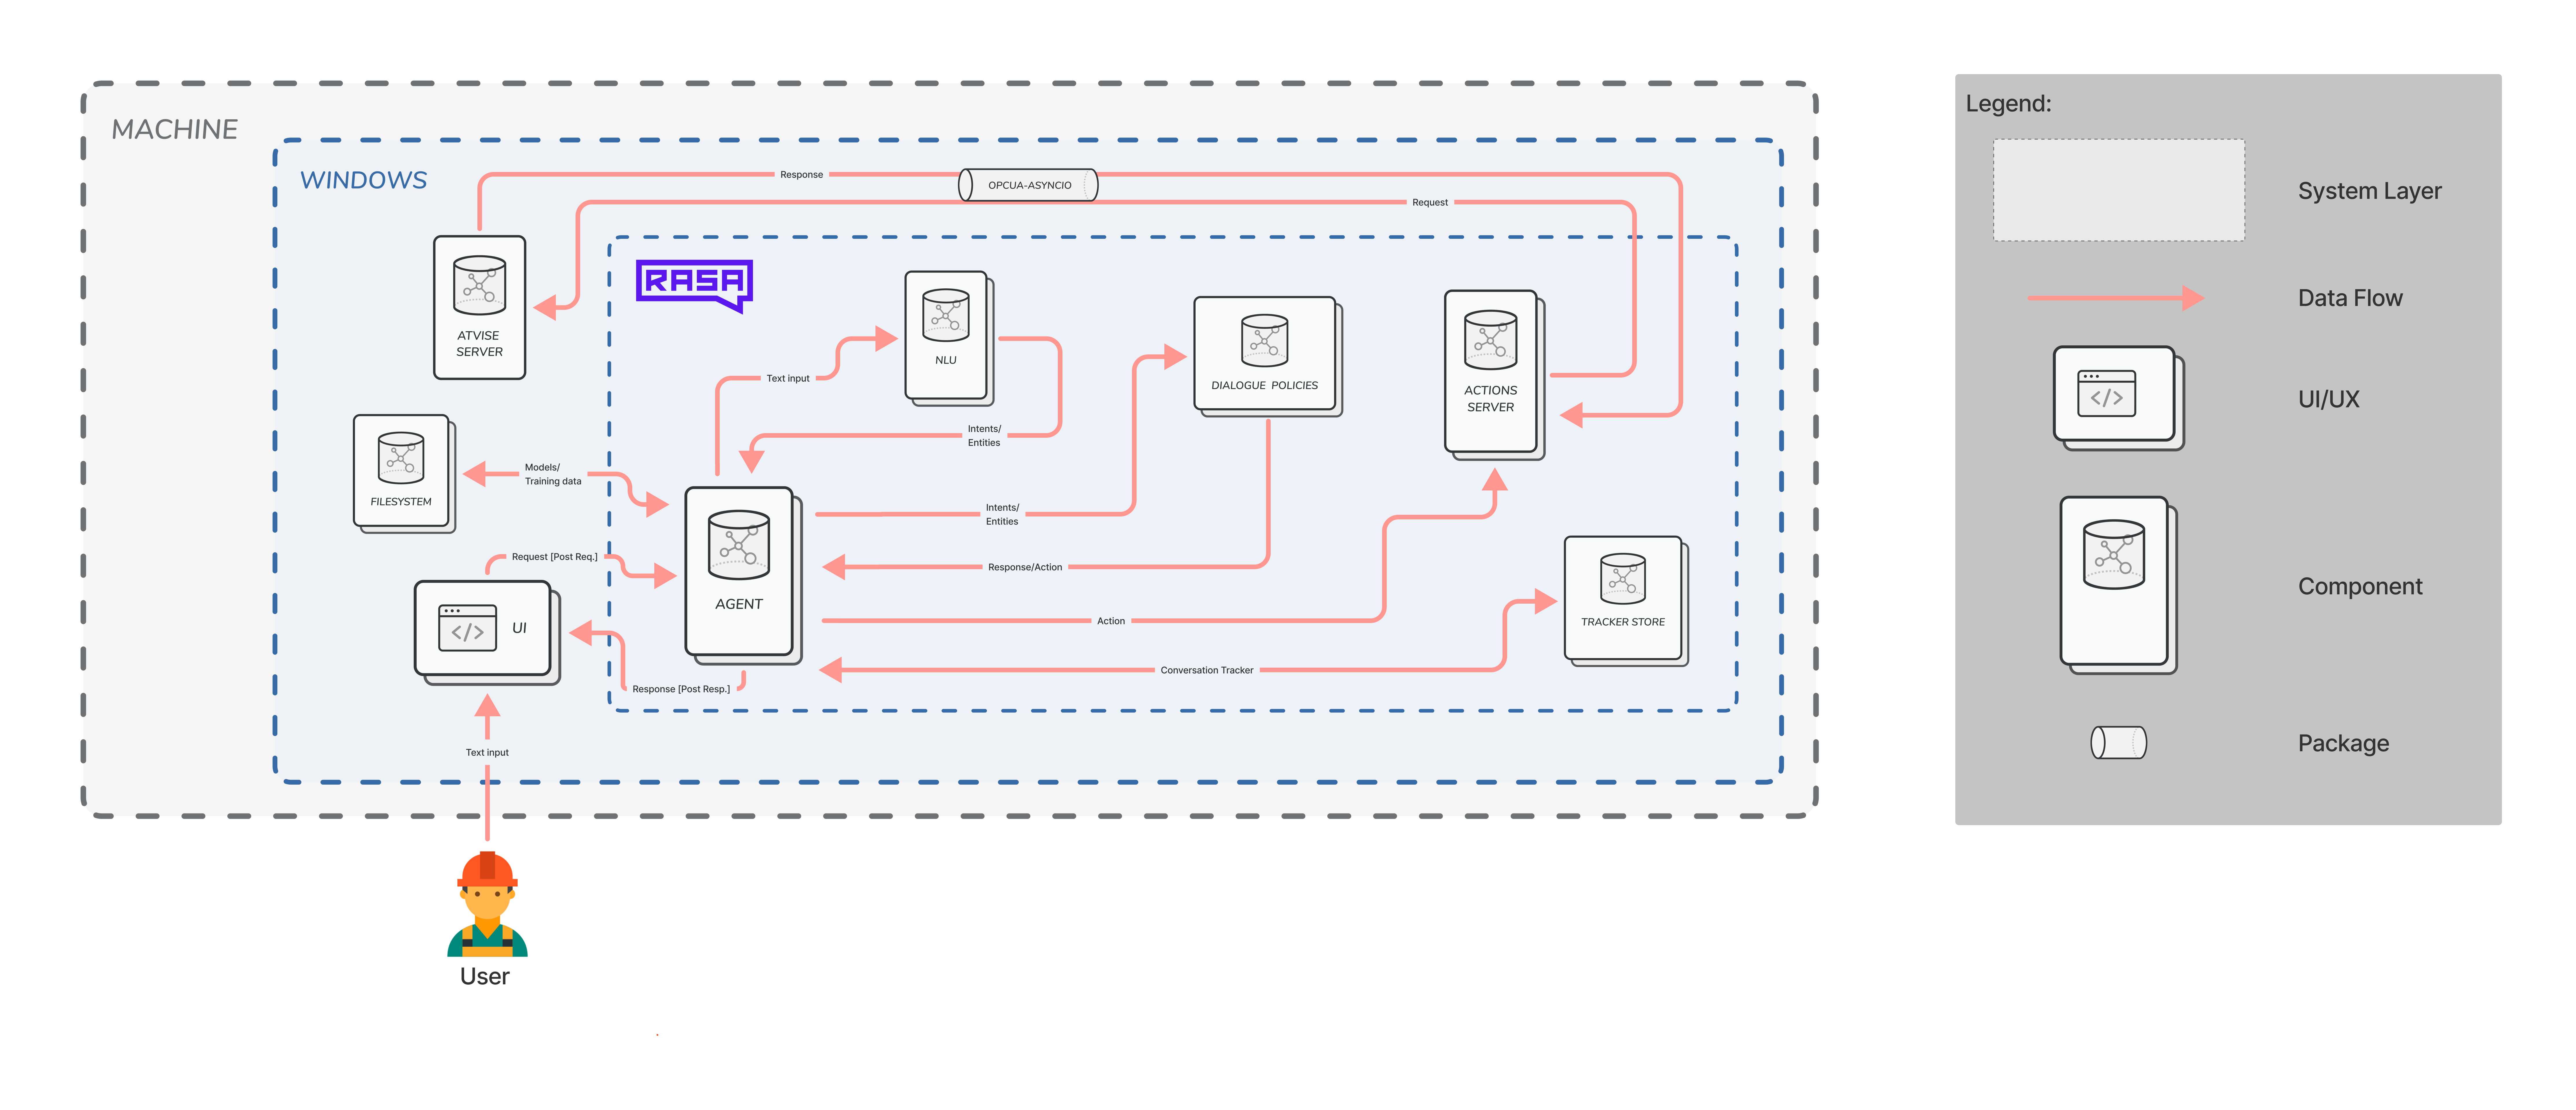
\includegraphics[width=0.95\linewidth]{images/design_of_project_concept.png}
\end{center}
}

%%%%%%%%%%%%%%%%%%%%%%%%%%%%%%%%%%%%%%%%%%%%%%%%%%%%%%%%%%%%%%%%%%%%%%%%%%%%%%
\headerbox{Details}{name=details,column=0, below=architecture}{
%%%%%%%%%%%%%%%%%%%%%%%%%%%%%%%%%%%%%%%%%%%%%%%%%%%%%%%%%%%%%%%%%%%%%%%%%%%%%%
To go further into detail, concerning the exact process of a chatbot interaction, one can have a look at the following sequence diagram.

\begin{center}
	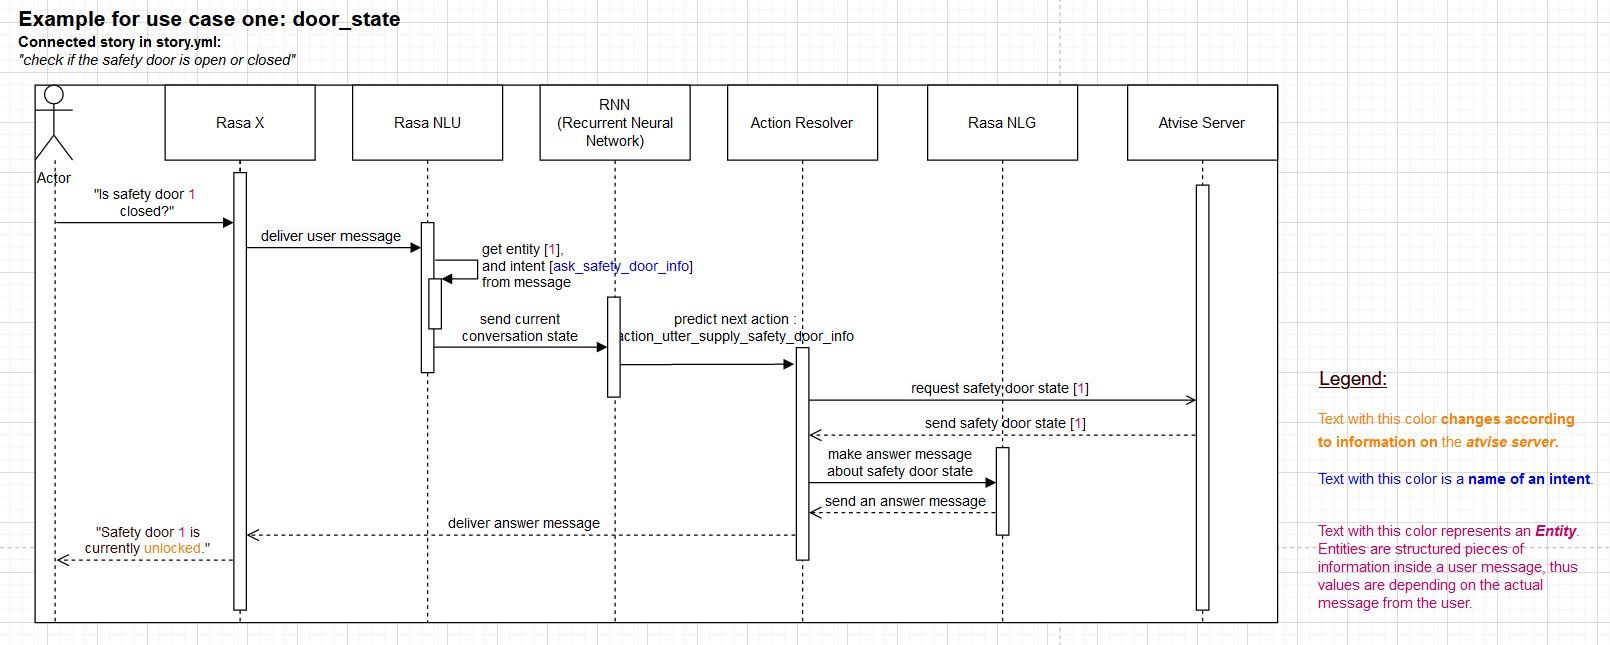
\includegraphics[width=1\linewidth]{images/sequence_diagram.jpg}
\end{center}

In this example a worker wants to know the state of a safety door on the machine. 
They input their command through Rasa X which is a chat UI already integrated into Rasa. 
The different components integrated into Rasa then take over and deciphers the user’s intent and extracts the exact door number. 
Next Rasa actions contacts the atvise server to find out about the specified safety door state. 
Finally, the answer is passed back to the worker.

}


%%%%%%%%%%%%%%%%%%%%%%%%%%%%%%%%%%%%%%%%%%%%%%%%%%%%%%%%%%%%%%%%%%%%%%%%%%%%%%
  \headerbox{Results}{name=results,column=1,span=1}{
%%%%%%%%%%%%%%%%%%%%%%%%%%%%%%%%%%%%%%%%%%%%%%%%%%%%%%%%%%%%%%%%%%%%%%%%%%%%%%
The talking machines team was able to implement the following use cases in English. \\

Simple state requests:
\begin{center}
	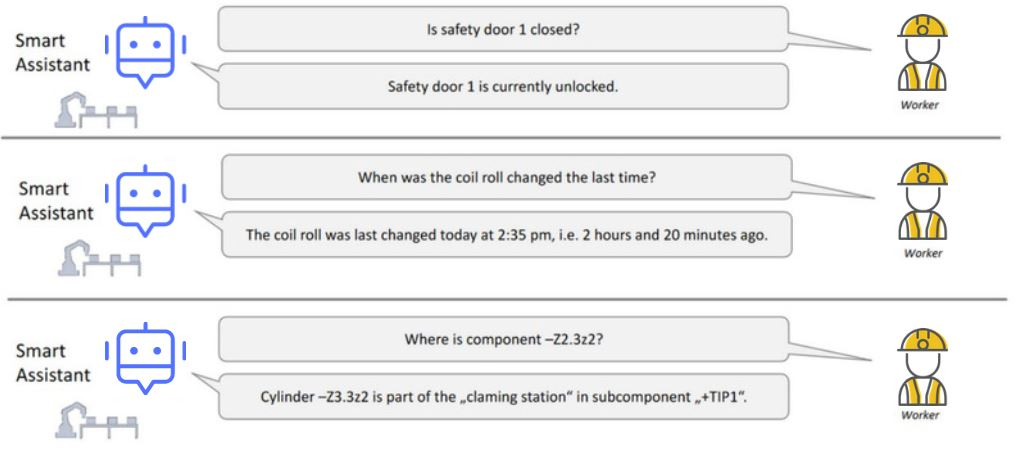
\includegraphics[width=0.85\linewidth]{images/use_case_1.jpg}
\end{center}
Proactive communication, optional continuations and processing contextual information:
\begin{center}
	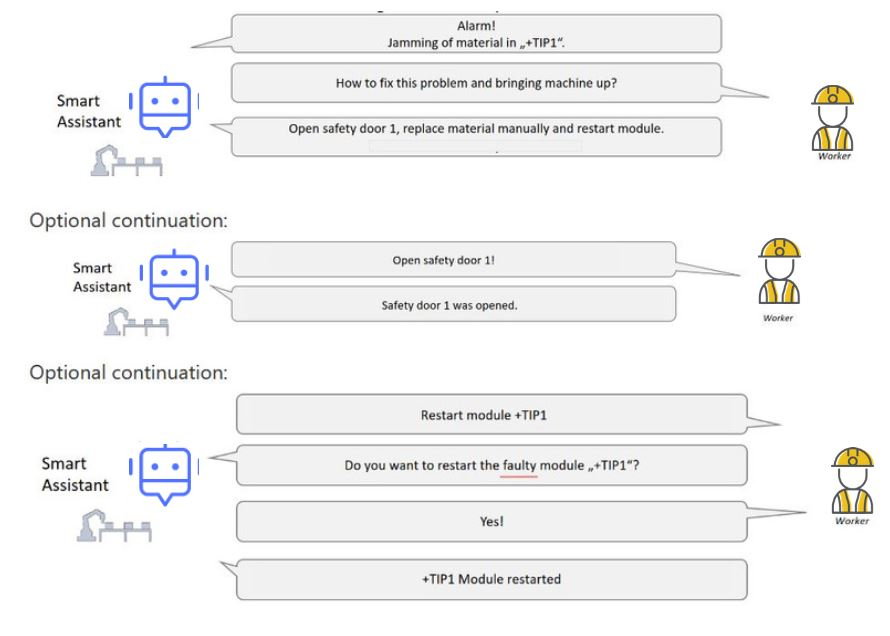
\includegraphics[width=0.85\linewidth]{images/use_case_2.jpg}
\end{center}
Proactive communication and processing contextual information:
\begin{center}
	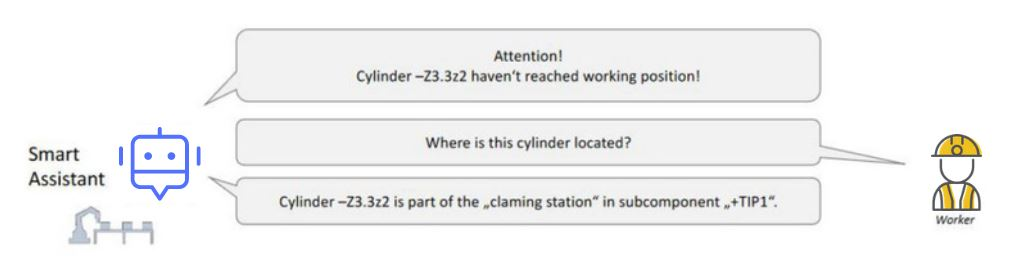
\includegraphics[width=0.85\linewidth]{images/use_case_3.jpg}
\end{center}
}

%%%%%%%%%%%%%%%%%%%%%%%%%%%%%%%%%%%%%%%%%%%%%%%%%%%%%%%%%%%%%%%%%%%%%%%%%%%%%%
\headerbox{Outlook}{name=outlook,column=1,span=1,below=results}{
  %%%%%%%%%%%%%%%%%%%%%%%%%%%%%%%%%%%%%%%%%%%%%%%%%%%%%%%%%%%%%%%%%%%%%%%%%%%%%%
  Next steps for the project could be implementing this prototype on a real Hekuma machine. 
  This would mean instead of just flipping values on the atvise server, interaction with the chatbot could move actual machine parts. 
  Implementation of this would require an adaptation of the current implementation to the specific machine. 
  For example, you would need to verify if information about the state of the machine is structured in a similar way as it is on our atvise server model. 
  Still, the overall architecture of the prototype would make this possible, as it is tightly fitted to the requirements of a Hekuma machine. \\

  Further, the prototype is effortlessly expandable. A variety of a new use cases can easily be implemented. \\

  A completely new feature to implement, could be multilingualism. We already developed a draft 
  for this during our time on the project, having a separate NLU for each desired language, as shown in the image. 
  \begin{center}
    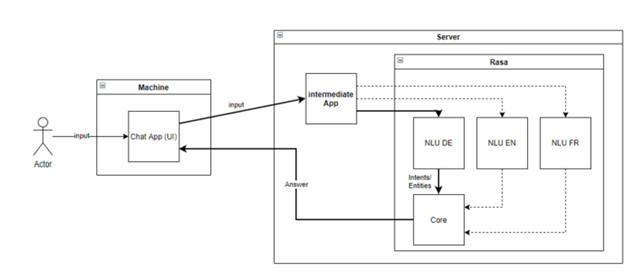
\includegraphics[width=0.8\linewidth]{images/multi_lang.png}
  \end{center}
}

%%%%%%%%%%%%%%%%%%%%%%%%%%%%%%%%%%%%%%%%%%%%%%%%%%%%%%%%%%%%%%%%%%%%%%%%%%%%%%
\headerbox{Team}{name=team,column=0, row=0, above=bottom}{
%%%%%%%%%%%%%%%%%%%%%%%%%%%%%%%%%%%%%%%%%%%%%%%%%%%%%%%%%%%%%%%%%%%%%%%%%%%%%%
\begin{center}
\begin{tabular}{cc}
	Saliu Bah &  Marco Lenz \\
	Cristina Vizan Olmedo & Jung Eun Park \\
\end{tabular}
\end{center}	
}
%%%%%%%%%%%%%%%%%%%%%%%%%%%%%%%%%%%%%%%%%%%%%%%%%%%%%%%%%%%%%%%%%%%%%%%%%%%%%%%
 
%%%%%%%%%%%%%%%%%%%%%%%%%%%%%%%%%%%%%%%%%%%%%%%%%%%%%%%%%%%%%%%%%%%%%%%%%%%%%%%
\headerbox{References}{name=references,column=1,span=1,above=bottom}{
  %%%%%%%%%%%%%%%%%%%%%%%%%%%%%%%%%%%%%%%%%%%%%%%%%%%%%%%%%%%%%%%%%%%%%%%%%%%%%%%
      \smaller
      \bibliographystyle{ieee}
      
      \begin{enumerate}
        \item Market Research Future. (2021, October). \emph{Voice Assistant Market Size, Share Forecast 2027}. https://www.marketresearchfuture.com/reports/voice-assistant-market-4003
        \item Petrock. (2020)  \emph{Voice Assistant and Smart Speaker Users 2020}. eMarketer. https://www.emarketer.com/content/voice-assistant-and-smart-speaker-users-2020#page-report
        \item Pistorius, J. (2020) \emph{Industrie 4.0 – vierte industrielle Revolution.} Springer Vieweg
      \end{enumerate}
      
     \vspace{0.3em}
}


\end{poster}

\end{document}

\grid
